
In 1997, Deep Blue, a supercomputer built by IBM, won a six games match against Garry Kasparov, the current world chess champion. Humans got beaten in Chess, but remain undefeated in other games. Consequently, researchers are looking for improvements in Artificial Intelligence.
\newline

The project is called \emph{Fast \& Furious Game Playing, Monte Carlo Drift}. Its purpose is to create an Artificial Intelligence able to compete against humans using the \emph{Monte Carlo Tree Search}.
\newline

The focus of this project is on two player strategy board games, while avoiding games already solved\footnote{A game solved is a game where good algorithms are able to find the perfect move in each situation to win, or to draw. For instance, \textit{Tic Tac Toe} or \textit{Draughts} are solved games.}. That is why this project is about the game \emph{Arimaa}.
\newline

To evaluate the best move, the algorithm develops a tree by creating nodes for all possible moves. Statistics are computed by evaluating these nodes and are results of a deeper exploration of a nodes. The algorithm would then be able to choose the best move according to it.
\smallbreak
\begin{figure}[!h] 
\centerline{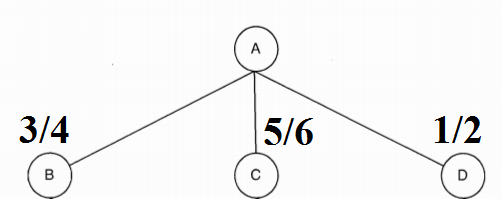
\includegraphics[scale=0.75]{1_Presentation/1.1_Our_project_Dan/tree}}
  \caption{An exploring tree : \newline The probabilities related to the nodes are the numbers, so the best node is the node B according to the statistics. See more in part  use \ref{trees}.} %centering caption
  \centering
\end{figure}
The \emph{Monte Carlo Tree Search} has been used in the past for \textit{Draughts}, or \textit{Chess}. It explores numerous random possibilities, and takes good decisions to win the game.
The algorithm would be parallelized in order to use it in a multi-core machine, allowing it to go further into the search tree, thus improving its efficiency.
\newline

Different parallelization methods will be studied in order to choose the most suitable, for this project.
The exploration of the tree will depend on the parallelization method.
The initial phase of the project would be the analysis of the latest papers concerning the technologies that might be of use.
The consecutive phases will be about making a choice among these technologies, to decide on the specifications.
\newline

Finally, in the last phase, a solution will be implemented, and executed on Grid'5000, a cluster of multi-core machines.
The interesting part about this project is the creation of an artificial intelligence as optimized as possible.


